\documentclass[11pt]{article}
\usepackage{graphicx}
\usepackage{enumerate}
\usepackage{subfigure}
\begin{document}
\title{Implement different DC topologies}
\author{Feng Wang}
\date{\today}
\maketitle
\section{My Work}
I implement DCell, Fat tree, FlattenedButterfly, HyperX, Long Hop and small-world (including SW Ring, SW 2-D Torus and SW 3-D Hexangonal Torus)using networkx. Although I have implemented fat tree before, I didn't use networkx then. So I decide to use networkx to draw it. Besides, I also use Simpy to implement ECMP on different topologies. As for F10, I use my old cpp codes to implment ``Wait and Hop'' on it.  
\section{DC topologies}

\subsection{DCell}
The left figure is $DCell_1$ in the paper. The number in red is the id of each switch or server. And I calculate the ID using the following formula which is also given in paper.
\[
uid_k = a_0 + \Sigma_{j=1}^{k}\{a_j \times t_{j-1}\}
\]
The number of severs in DCell is $n$ times than that of switches since each switch connects $n$ servers. So, the IDs of switches will be between Max\_Server\_ID+1 and Max\_Server\_ID+Number\_of\_Servers/$n$, which is [20,24] in this example.\vspace{2ex}\\
The right figure is created using networkx. The nodes in write is Mini-switches and the servers are red. For simplicity, I take $n = 4$ and $k = 1$ here. \vspace{2ex}\\
\begin{itemize}
	
	\item
	\centerline{}
	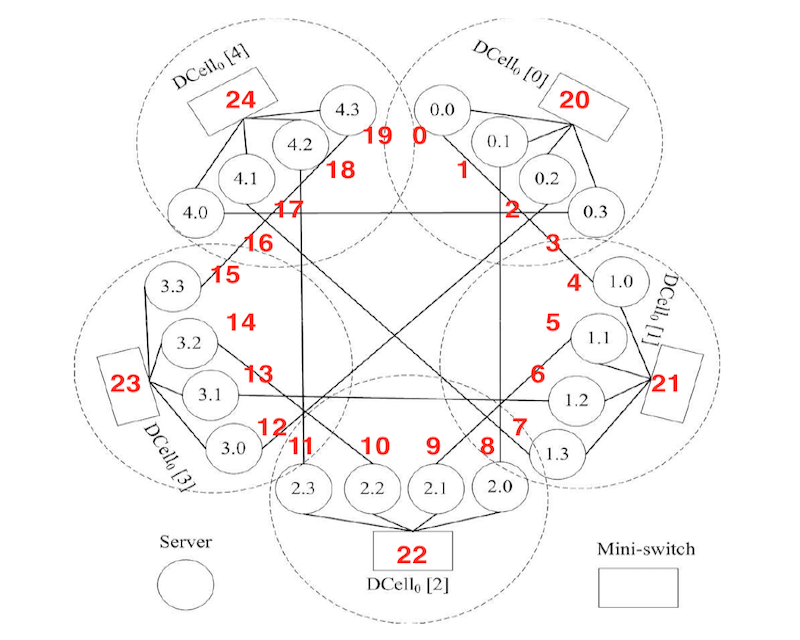
\includegraphics[width=0.4\textwidth]{figure/draw/DCell_original.png}
	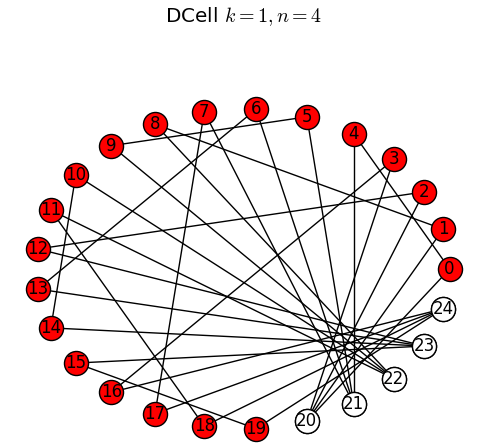
\includegraphics[width=0.4\textwidth]{figure/draw/DCell.png}
	
\end{itemize}

I generate flows with random destinations for all the nodes in this topology. Actually, for all the following topologies, I implement the ECMP in the same way. The process which is responsible for generating flows is a Poisson process, where $\lambda = 0.1$. The size of each flow is uniformly distributed between 1 and 100 bits. The capacity is 100bps for each link, so the average completion time of each flow will not be very small. Apparently, 100bps is not the practical number. However, it doesn't matter since I focus on the comparison now. Meanwhile, all the flows share the same link sending rate and I assume all the switches have infinite buffer size. It is very basic and simple currently, but I can add more advanced features later. I will not repeat these details in the remaining topologies. The next figure is the average completion time of each flow of 100 trials. \\
\centerline{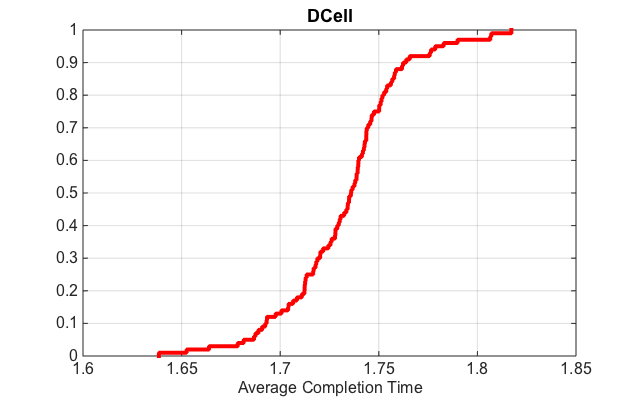
\includegraphics[width=0.5\textwidth]{figure/picture/DCell.png}}



\subsection{Flattened Butterfly}
The topology: \\
\begin{itemize}
	\item \centerline{}
	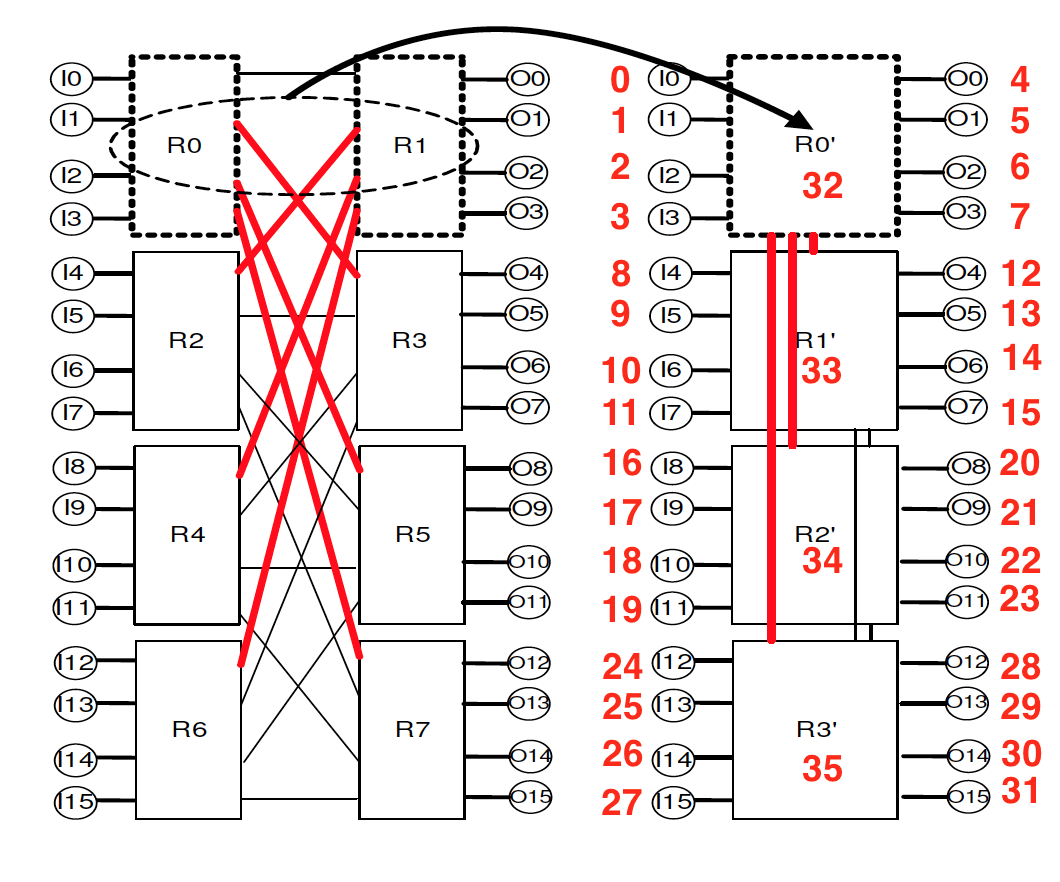
\includegraphics[width=0.5\textwidth]{figure/draw/FlattenedButterfly_original.png}
	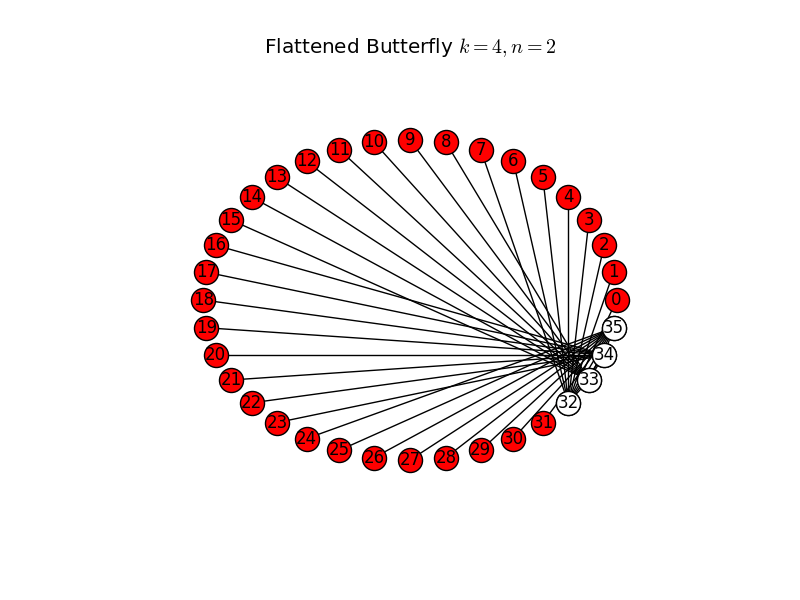
\includegraphics[width=0.5\textwidth]{figure/draw/FlattenedButterfly.png}
	
\end{itemize}
The average completion time: \\
\centerline{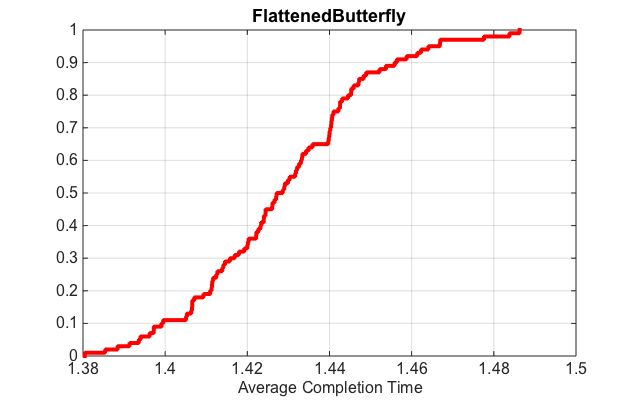
\includegraphics[width=0.5\textwidth]{figure/picture/FlatenedButterfly}}


\subsection{HyperX}

The average completion time: \\
\centerline{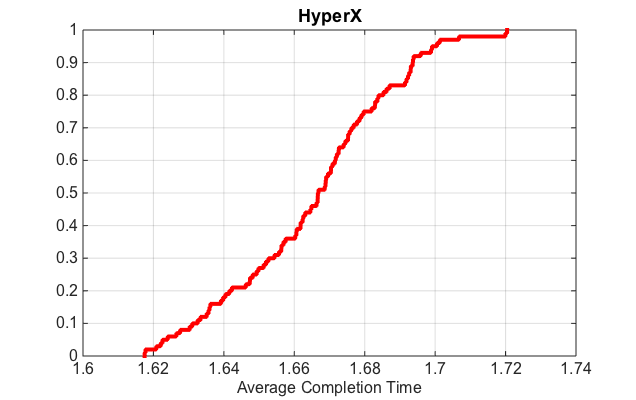
\includegraphics[width=0.5\textwidth]{figure/picture/HyperX.png}}
The toplogy: 
\begin{itemize}
	\item \centerline{}
	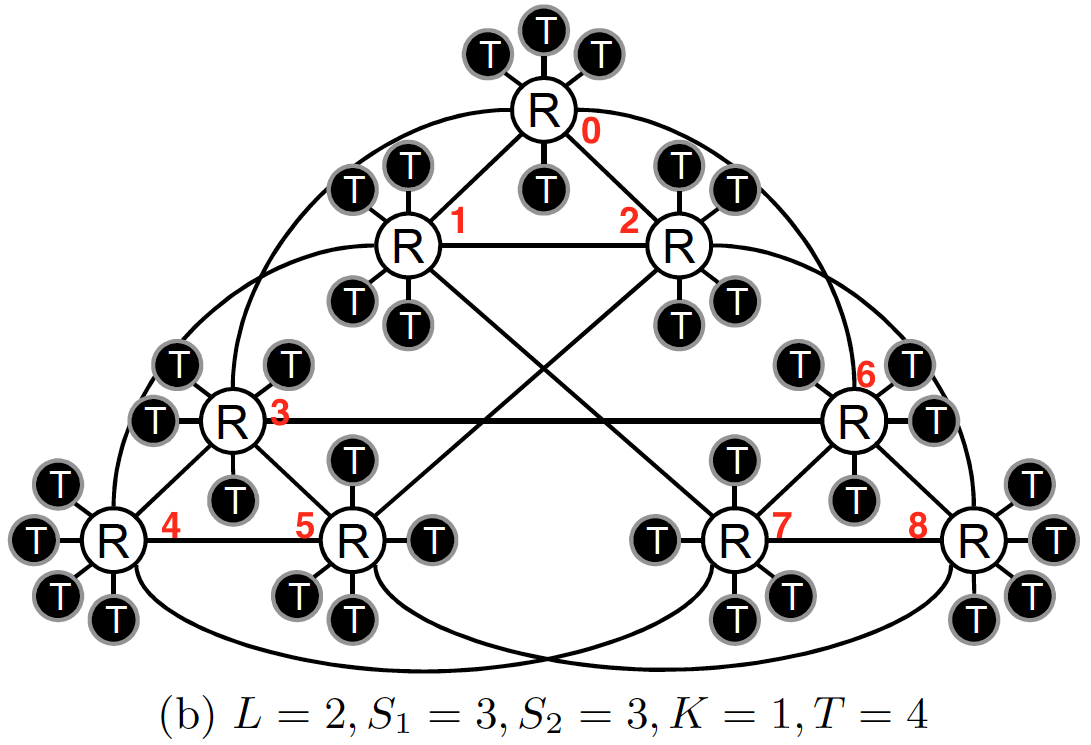
\includegraphics[width=0.5\textwidth]{figure/draw/HyperX_original}
	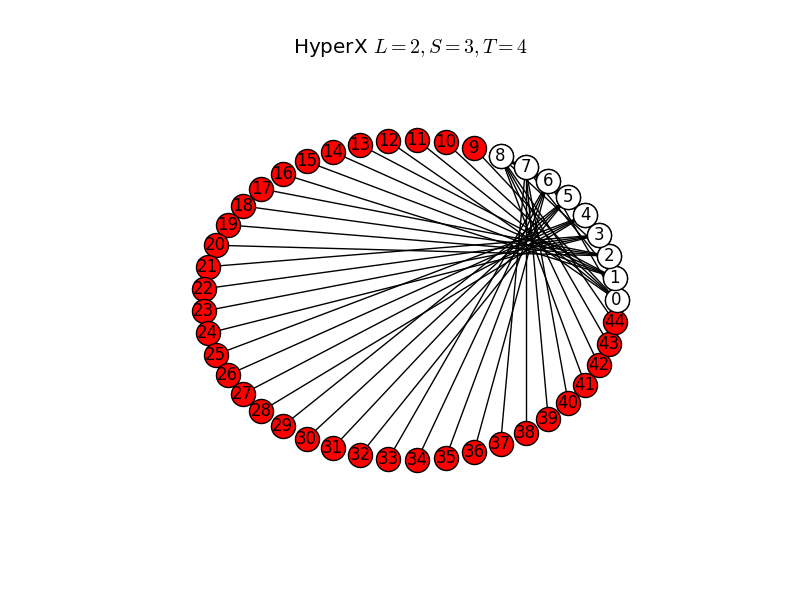
\includegraphics[width=0.5\textwidth]{figure/draw/HyperX.png}
\end{itemize}

\subsection{F10}

The average completion time (ECMP):\\
\centerline{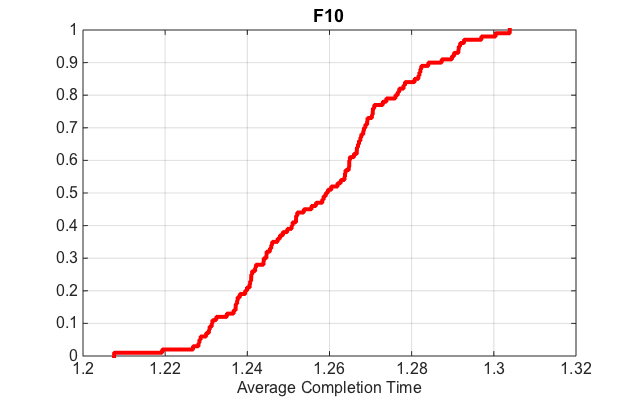
\includegraphics[width=0.5\textwidth]{figure/picture/F10.png}}
The average completion time (Wait and Hop):\\
\centerline{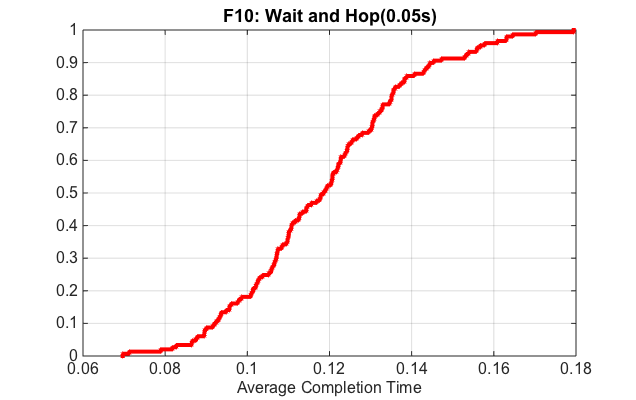
\includegraphics[width=0.5\textwidth]{figure/picture/F10_wait_and_hop.png}}
The topology shown in paper and implemented using networkx: \\
\begin{itemize}
	\item \centerline{}
	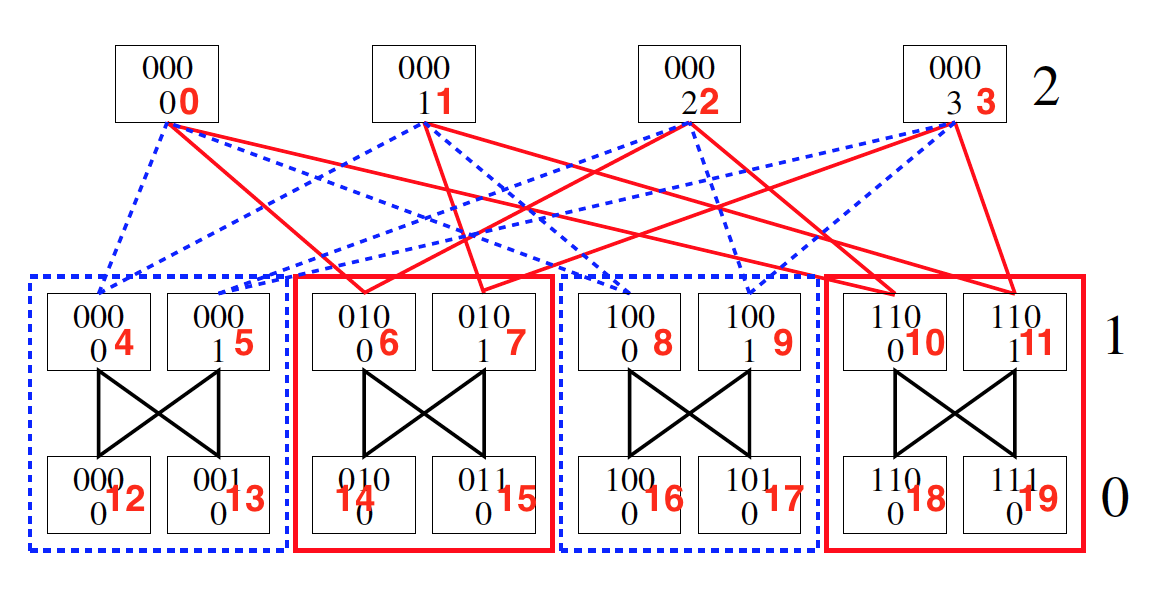
\includegraphics[width=0.5\textwidth]{figure/draw/F10_original}
	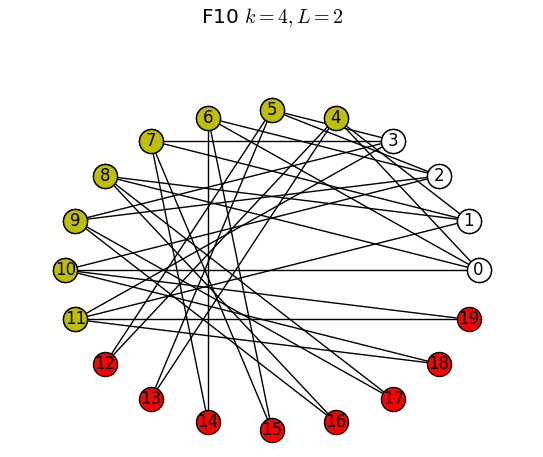
\includegraphics[width=0.5\textwidth]{figure/draw/F10.png}
\end{itemize}

\subsection{Long Hop}
Long Hop is the most difficult one. Suppose we have $N$ switches where $N = 2^d$  and each switch has $m$ ports. Then we can use $d$ binary digits to represent all the nodes. For given $d$ and $m$, this topology uses the \emph{generator metrix} $G$ over GF(2). $G$ has a standard form $G = (I_d | P)$ and $P$ is some $d \times (m-d)$ matrix.\vspace{2ex}\\
This paper doesn't give any figure of Long Hop topology...... The following figure is one example where $d=4$ and $m=5$

\centerline{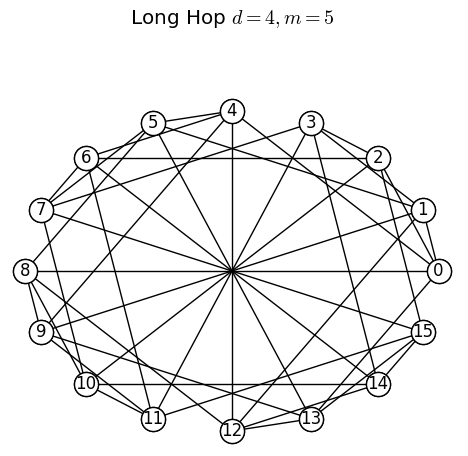
\includegraphics[width=0.5\textwidth]{figure/draw/LongHop}}

\subsection{Small-World}
The blue lines are random links. The SW 3-D has too many links, I only draw the blue links. The networkx can generate small world topologies actually, but it's different. The small world in DCs has some constrain, for example limiting the degree of each node to 6. 
\subsubsection{SW Ring}
The average completion time: \\
\centerline{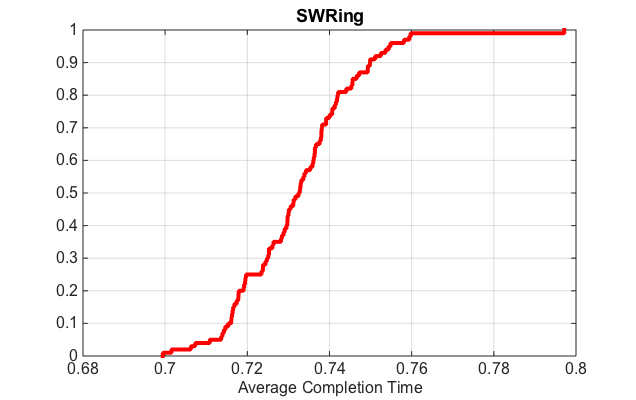
\includegraphics[width=0.5\textwidth]{figure/picture/SWRing.png}}
In this topology, all the nodes can randomly connect 4 other 
\begin{itemize}
	\item \centerline{}
	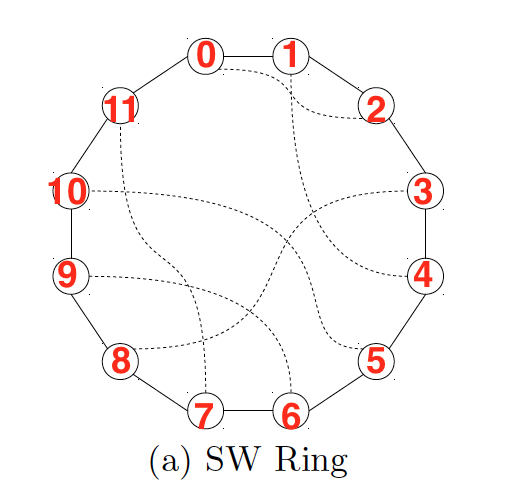
\includegraphics[width=0.45\textwidth]{figure/draw/SWRing_original}
	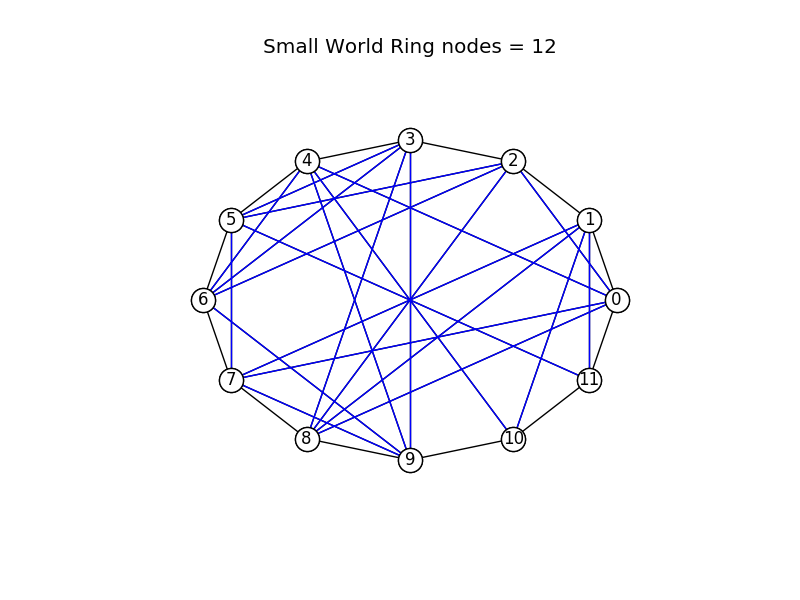
\includegraphics[width=0.55\textwidth]{figure/draw/SWRing.png}
\end{itemize}

\subsubsection{SW 2D}
The average completion time: \\
\centerline{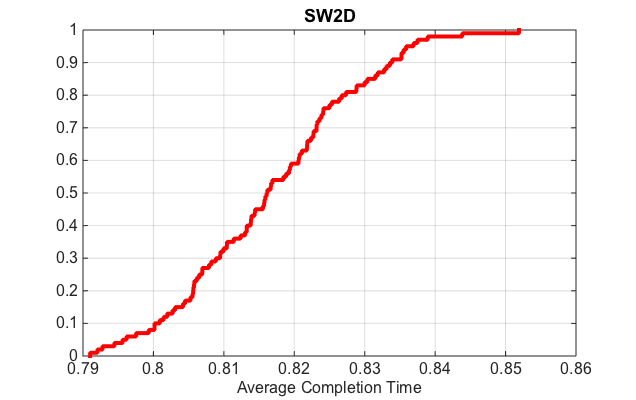
\includegraphics[width=0.5\textwidth]{figure/picture/SW2D.png}}
The topology:
\begin{itemize}
	\item \centerline{}
	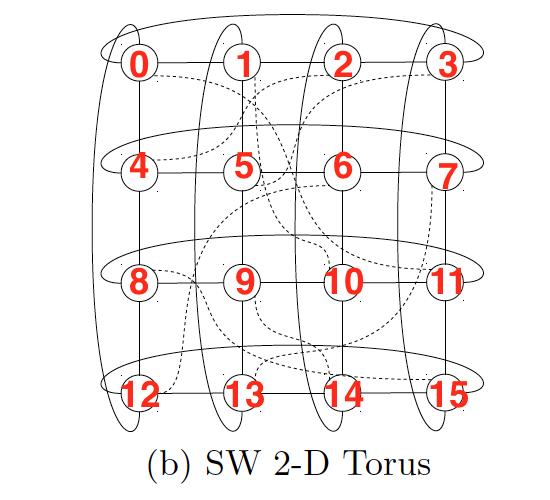
\includegraphics[width=0.45\textwidth]{figure/draw/SW2D_original}
	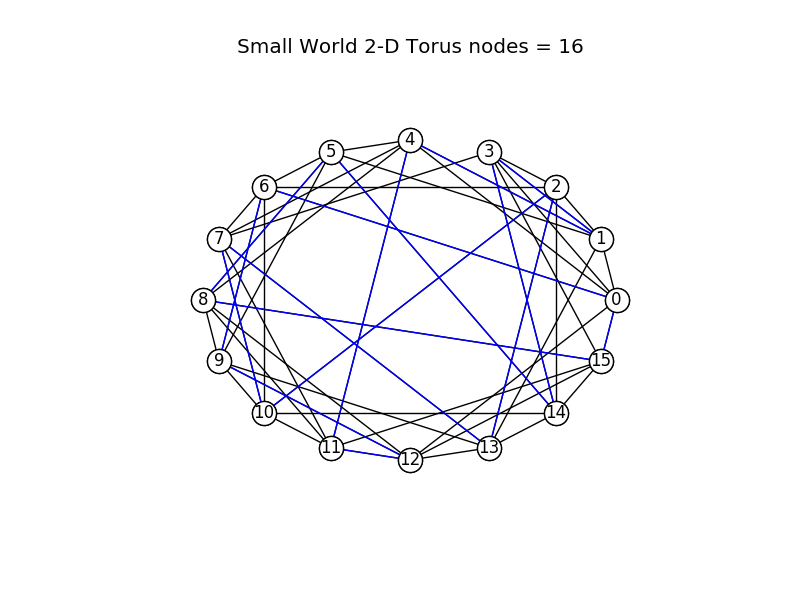
\includegraphics[width=0.55\textwidth]{figure/draw/SW2D.png}
\end{itemize}

\subsubsection{SW 3D}
The average completion time: \\
\centerline{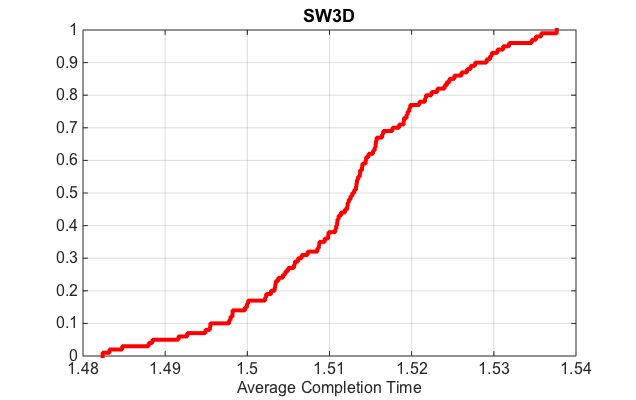
\includegraphics[width=0.5\textwidth]{figure/picture/SW3D.png}}
The nodes in first dimension is ranging from 0 to 23, nodes in second dimension is ranging from 24 to 47 and the range of the last is [48,71]. There are totally 72 nodes here. 
\begin{itemize}
	\item \centerline{}
	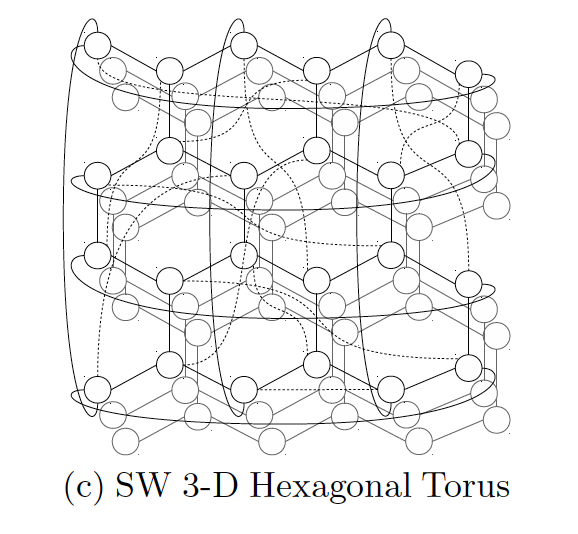
\includegraphics[width=0.5\textwidth]{figure/draw/SW3D_original}
	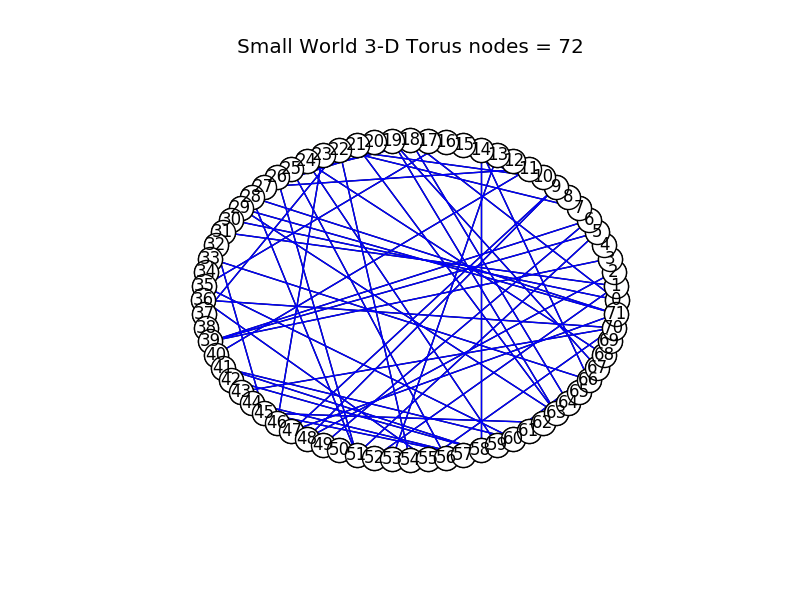
\includegraphics[width=0.5\textwidth]{figure/draw/SW3D.png}
\end{itemize}

\section{Analysis and Summary}
I put CDFs of average completion time together\\
\centerline{\includegraphics[width=0.6\textwidth]{figure/picture/All_new.png}}
The SWRing takes the least time because many nodes are directly connected. Intuitively, SW2D and SW3D will take more time than SWRing. The figure shows flows in DCell have the longest survival time. It is interesting to see that there is a big gap between Long hop and F10. Considering there are many uncertainties in this experiment (random flow sizes, random links), the results shown above may not very accurate, but I think it is relatively reasonable. 

\end{document}
